Given a boolean formula in NAE3SAT form, 

\chapter{Decidability Problems for Hinged Polygons and Disks}
\section{The Logic Engine}
#History of the logic engine.  Who invented it [comsadkis???]?
\subsection{Construction of the Logic Engine and Encoding of an NAE3SAT Problem on a Logic 
Engine}
%#idea: SEPARATE THE CONSTRUCTION FROM THE REPRESENTATION.  AFTERWARDS TIE THE CONSTRUCTION TO 
%#REPRESENTATION
%#rigid frame - define as units of height in terms of n,m, and flag sizes (clauses, variables, and 
%#the size of qeqquilateral triangle.  the rigid frame does not move  {(x,y) | rigid frame 
%#dimensions}

# shaft {x | 0 <=x <= xMax}


\begin{figure}[!h]
\begin{center}
%%%First Figure with armatures
\includegraphics{graphics/LogicEngineFrameFigure1Scaled.pdf}
\caption{A logic engine frame with veritical armatures and a horizontal 
shaft.}\label{fig:LogicEngineFrameFigure1.pdf}
\end{center}
\end{figure}


The logic engine is a planar model which can encode instances of the NAE3SAT problem.  The 
components of the logic engine are as follows: the rigid frame, the shaft, the armatures,
the chains, and the flags.  Figure \ref{fig:LogicEngineFrameFigure1.pdf} shows the a rigid frame, 
armatures, and shaft.  Each armature represents a boolean variable.  The rigid frame defines the border 
of the model and the armatures has two orientations with respect to the shaft.  
\begin{figure}[!h]
\begin{center}
\includegraphics{graphics/LogicEngineFrameFigure2Scaled.pdf}
\caption{}\label{fig:LogicEngineFrameFigure2.pdf}
\end{center}
\end{figure}
Flagging arragement indicates the relationship of the boolean literal's existence within a clause.  
There are two literals for each variable.  
\begin{enumerate}
 \item If the literal $x_j$ is found in clause $C_k$, then $l_{j,k}$ is unflagged.
 \item If the literal $\bar{x}_j$ is found in clause $C_k$, then $\bar{l}_{j,k}$ is unflagged.
\end{enumerate}
Negated literals reside below the shaft and non-negated literals reside above the shaft.
% If the NAE3SAT problem contains $m$ clauses, each armature is partitioned into $2m$ pieces.  Since the armatures represent the boolean variables, the corresponding l  $m$ pieces above the shaft and $m$ pieces below the shaft.  Each row at height $h$ above and below the shaft represents the $h^\text{th}$ clause in the boolean formula.  The flags indicate that the literal of the boolean variable does not occur in the clause, i.e.

A \textit{collision} of flags occur if either of the following occurs:
\begin{enumerate}
\item flags in the same row on adjacent armatures point toward each other.
\item a flag from the outermost armature $A_n$ points towards the outer rigid frame.
\item a flag from the innermost armature $A_1$ points inwards of $A_1$.
\end{enumerate}
\begin{figure}[!htbp]
\begin{center}
\includegraphics{graphics/logicEngineCollisions.pdf}
\caption{(a) Illustrates a adjacent flag collision at the same height, (b) and (c) illustrates a 
rigid frame collision.}\label{fig:logicEngineCollisions.pdf}
\end{center}

\end{figure}
\begin{figure}[!htbp]
\begin{center}
\includegraphics{graphics/logicEngineValidConfigurations.pdf}
\caption{The following configuration of adjacent flags 
and flags that are adjacent to the rigid frame.}\label{fig:logicEngineValidConfigurations.pdf}
\end{center}
\end{figure}
%define what it means to be collision-free
%explain why at least one armature is unflagged in every row.
%A row is said to be \textit{collistion-free} when 
\begin{lem}\label{lem:logicEngine1}A row has a collision-free configuration if and only if it has 
at least one unglagged armature. \end{lem}
\begin{proof}
% Do this by induction  start with 1, then suppose i flags point right, show the i+1 armature points 
% the to right.  State which types of collisions occur in the lemma.

Suppose all armatures are flagged in a row.  The flag on armature $A_1$ must point to the 
right otherwise we result in a rigid frame collision.  $A_2$ must point to the right otherwise 
we result in a rigid frame collision.  Without loss of generality, $A_i$ and $A_{i+1}$ must 
point to the right in order to prevent an adjacent flag collision.  This implies that $A_n$ 
must also point to the right which results into a rigid frame collision.
%The adjacent flags must point right as %well, i.e. $A_2, ..., A_n$.  The flag on $A_n$ 
% collides with the rigid frame.  
A same argument holds with the argument beginning with the flag 
on the armature $A_n$ pointing to the left.  Thus there is no collision-free configuration with 
all 
armatures flagged.

%Now suppose we unflag one armature, $A_i$.  By pointing all flags left of $A_i$ to the right and  
%point all flags right of $A_i$, each adjacent pair of flags have a valid configuration that is 
%collision-free.

Suppose there is an unflagged armature in a row.  Turn all flags towards the nearest unflagged 
armature.  If there are flags on $A_1$ and $A_n$, point toward the interior thus they do not 
collide with the 
rigid frame.  If there are flags on two consecutive armatures, they do not collide because the 
nearest unflagged armature cannot be between them.  Therefore the row has a collision-free 
configuration.
\end{proof}

\begin{figure}[!htbp]
\begin{center}
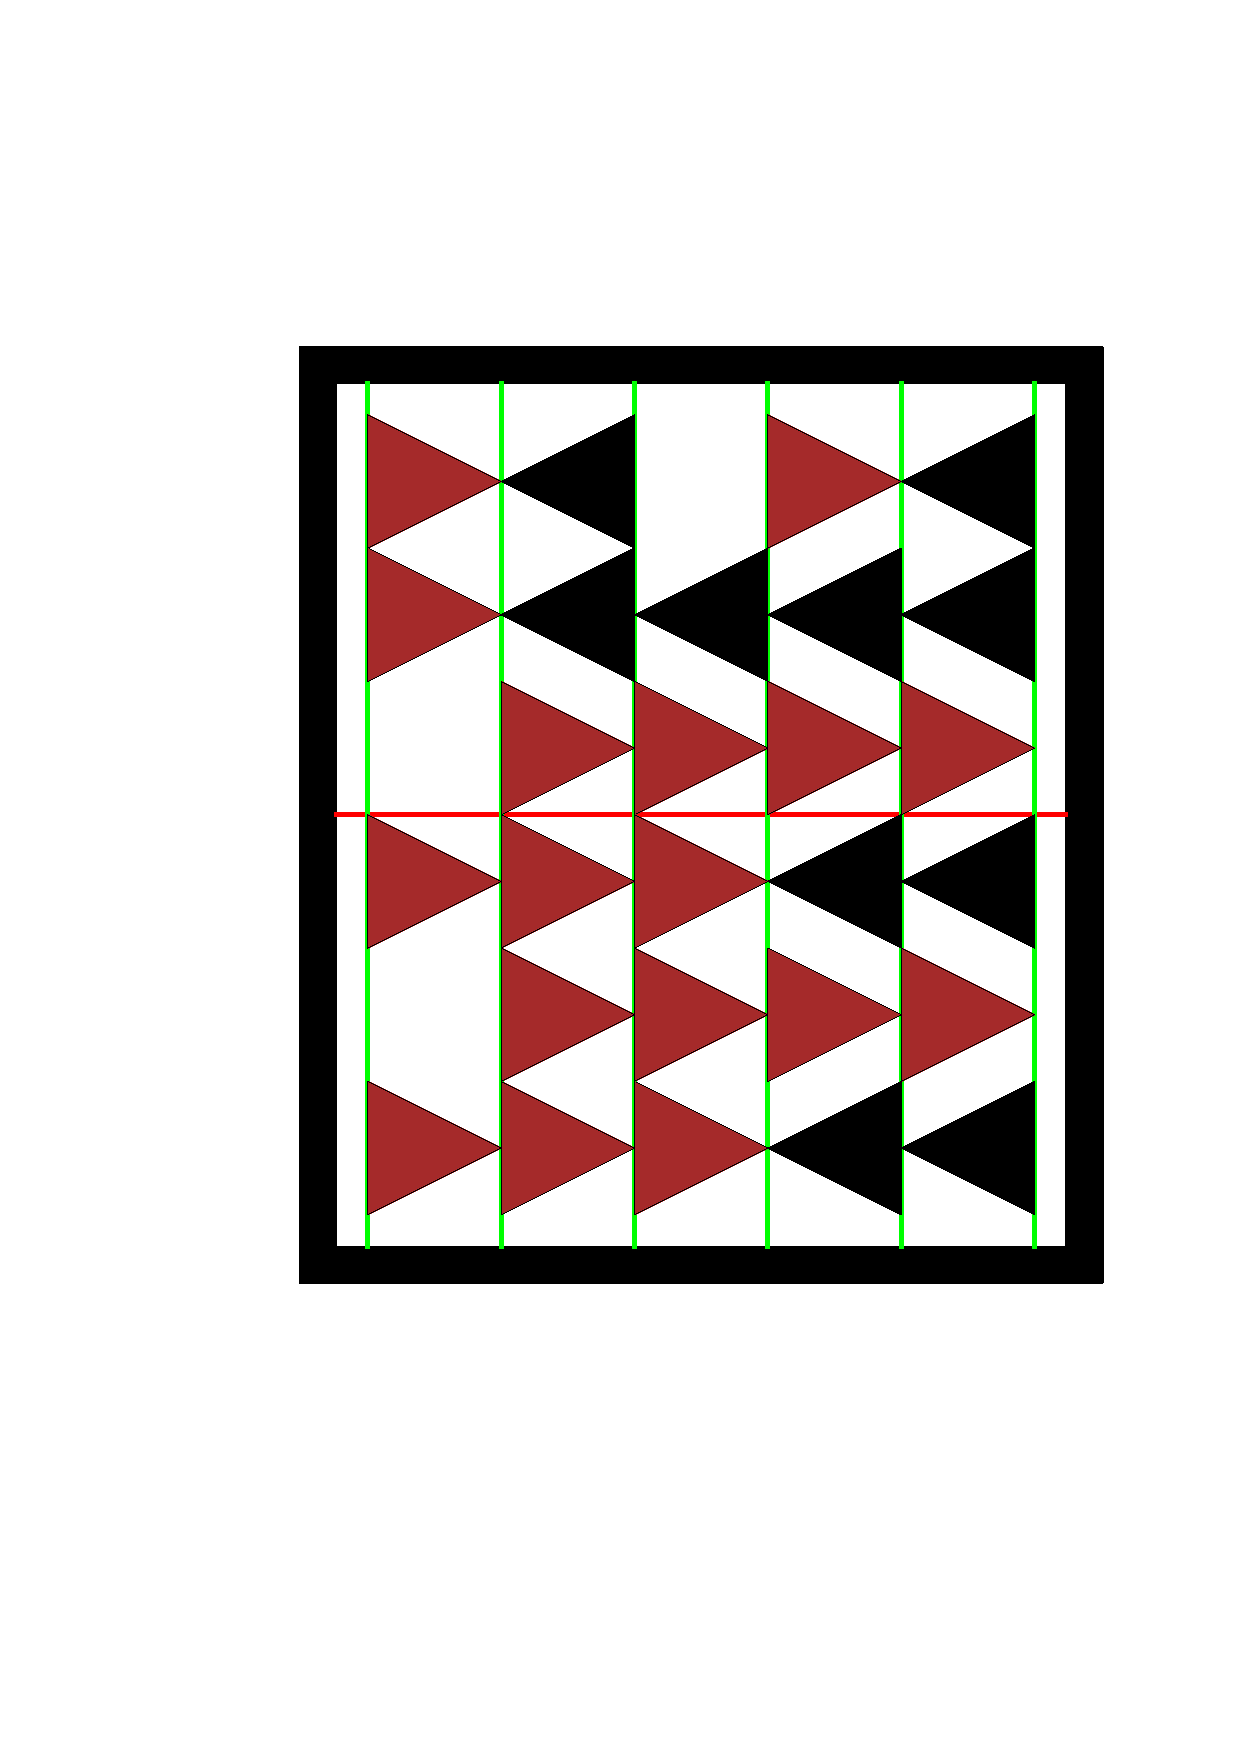
\includegraphics{graphics/LogicEngineFrameFigure5.pdf}
\caption{The logic engine from figure \ref{fig:LogicEngineFrameFigure2.pdf} whose armatures are rotated}\label{fig:LogicEngineFrameFigure5.pdf}
\end{center}
\end{figure}

%Add some introductory sentence of what happens next.  

\begin{thm}\label{thm:Satisfiability-1}
 Given an instance of a $NAE3SAT$,  it is a ``yes'' instance if and only if the 
corresponding logic engine has a collision-free configuration.
\end{thm}
\begin{proof}
Suppose we have an instance of a $NAE3SAT$ that is a ``yes'' instance. This implies that there is a 
truth assignment such that each clause contains a true and a false literal. Now consider the logic 
engine corresponding to this instance. We now 
show that it has a collision free configuration.

For variables that are true, configure the armatures such that the flags corresponding to the 
non-negated literals reside above the 
shaft and the flags that correspond to the negated literals reside below this shaft.  For variables 
that are false, configure the 
armatures in the opposite orientation.  Each clause corresponds to a pair of rows in 
the logic engine, one row for non-negated literals and one for negated literals.  Because the 
$NAE3SAT$ is a yes instance, every row contains at least one unflagged armature.  
By Lemma \ref{lem:logicEngine1}, every row  has a collision-free configuration.

Suppose we have an instance of a $NAE3SAT$ such that the corresponding logic engine has a 
collision-free configuration. By Lemma \ref{lem:logicEngine1} every row at least one unflagged 
armature.  The $k^{th}$ clause is represented by the $k^{th}$ rows above and below the shaft. If the 
literal $x_j$ is found in clause $C_k$, then the armature is unflagged in that row. If the literal 
$\bar{x}_j$ is found in clause $C_k$, then $\bar{l}_{j,k}$ is unflagged.  All flags 
corresponding to negated literals reside below the shaft and flags corresponding to non-negated 
literals reside above the shaft.  All together we have that every clause has a true literal and a 
false literal.  Thus, we have a 'yes' instance of the $NAE3SAT$.
%1) A collision-free configuration implies that every row at least one unflagged armature.
%  \item If the literal $x_j$ is found in clause $C_k$, then $l_{j,k}$ is unflagged.
%  \item If the literal $\bar{x}_j$ is found in clause $C_k$, then $\bar{l}_{j,k}$ is unflagged.
%  all negated literals reside below the shaft and non-negated literals reside above the shaft.
%  The k_th clause is represented by the k_th rows above and below the shaft.  This indicated that there is a negated and non-negated literal in each clause.  And so we have a 'yes' instance
%
%We assign true or false values to the variables.  If the 
%corresponding armatures 
%There is a truth assignment $t$
% t: A -> {1,0} s.t. for any C_j contains a true literal and a false literal.
%
%
% Given the corresponding logic engine has a flat, collision-free configuration for a $NAE3SAT$ 
% instance.  Then every row must have an unflagged armature.  Each clause has two corresponding rows, 
% one row for negated literals and one for non-negated literals.  Unflagged armatures implies the 
% existence of a literal in a clause. All together, this implies that every clause contains a true and 
% false literal.  Thus we have a ``yes'' $NAE3SAT$ instance.
\end{proof}

\section{Construction of the NAE3SAT Problem over Hinged Polygons}         
\begin{figure}[!htbp]
\begin{center}
\includegraphics{graphics/HingedLogicEngineSmall.pdf}
\caption{The logic engine realized as a polygonal linkage.}\label{fig:HingedLogicEngineSmall.pdf}
\end{center}
\end{figure}
\section{Construction of the NAE3SAT Problem over Disks}
%show the snowflake graph with just lines, then show the snowflake graph with the disks specifying 
%the size of the disks on the trunk and branches.  Then show the problem/proof using the Hausdorff 
%Distance